\chapter{Implementation}\label{ch:implementation}
To fulfill the assumptions of this work, the authors prepared a system that is able to collect and verify the mouse dynamics data.
The high-level flow of the system is presented in Fig.~\ref{fig:overall_system_structure} and provides the basis for further considerations.
\begin{figure}[!hbt]
    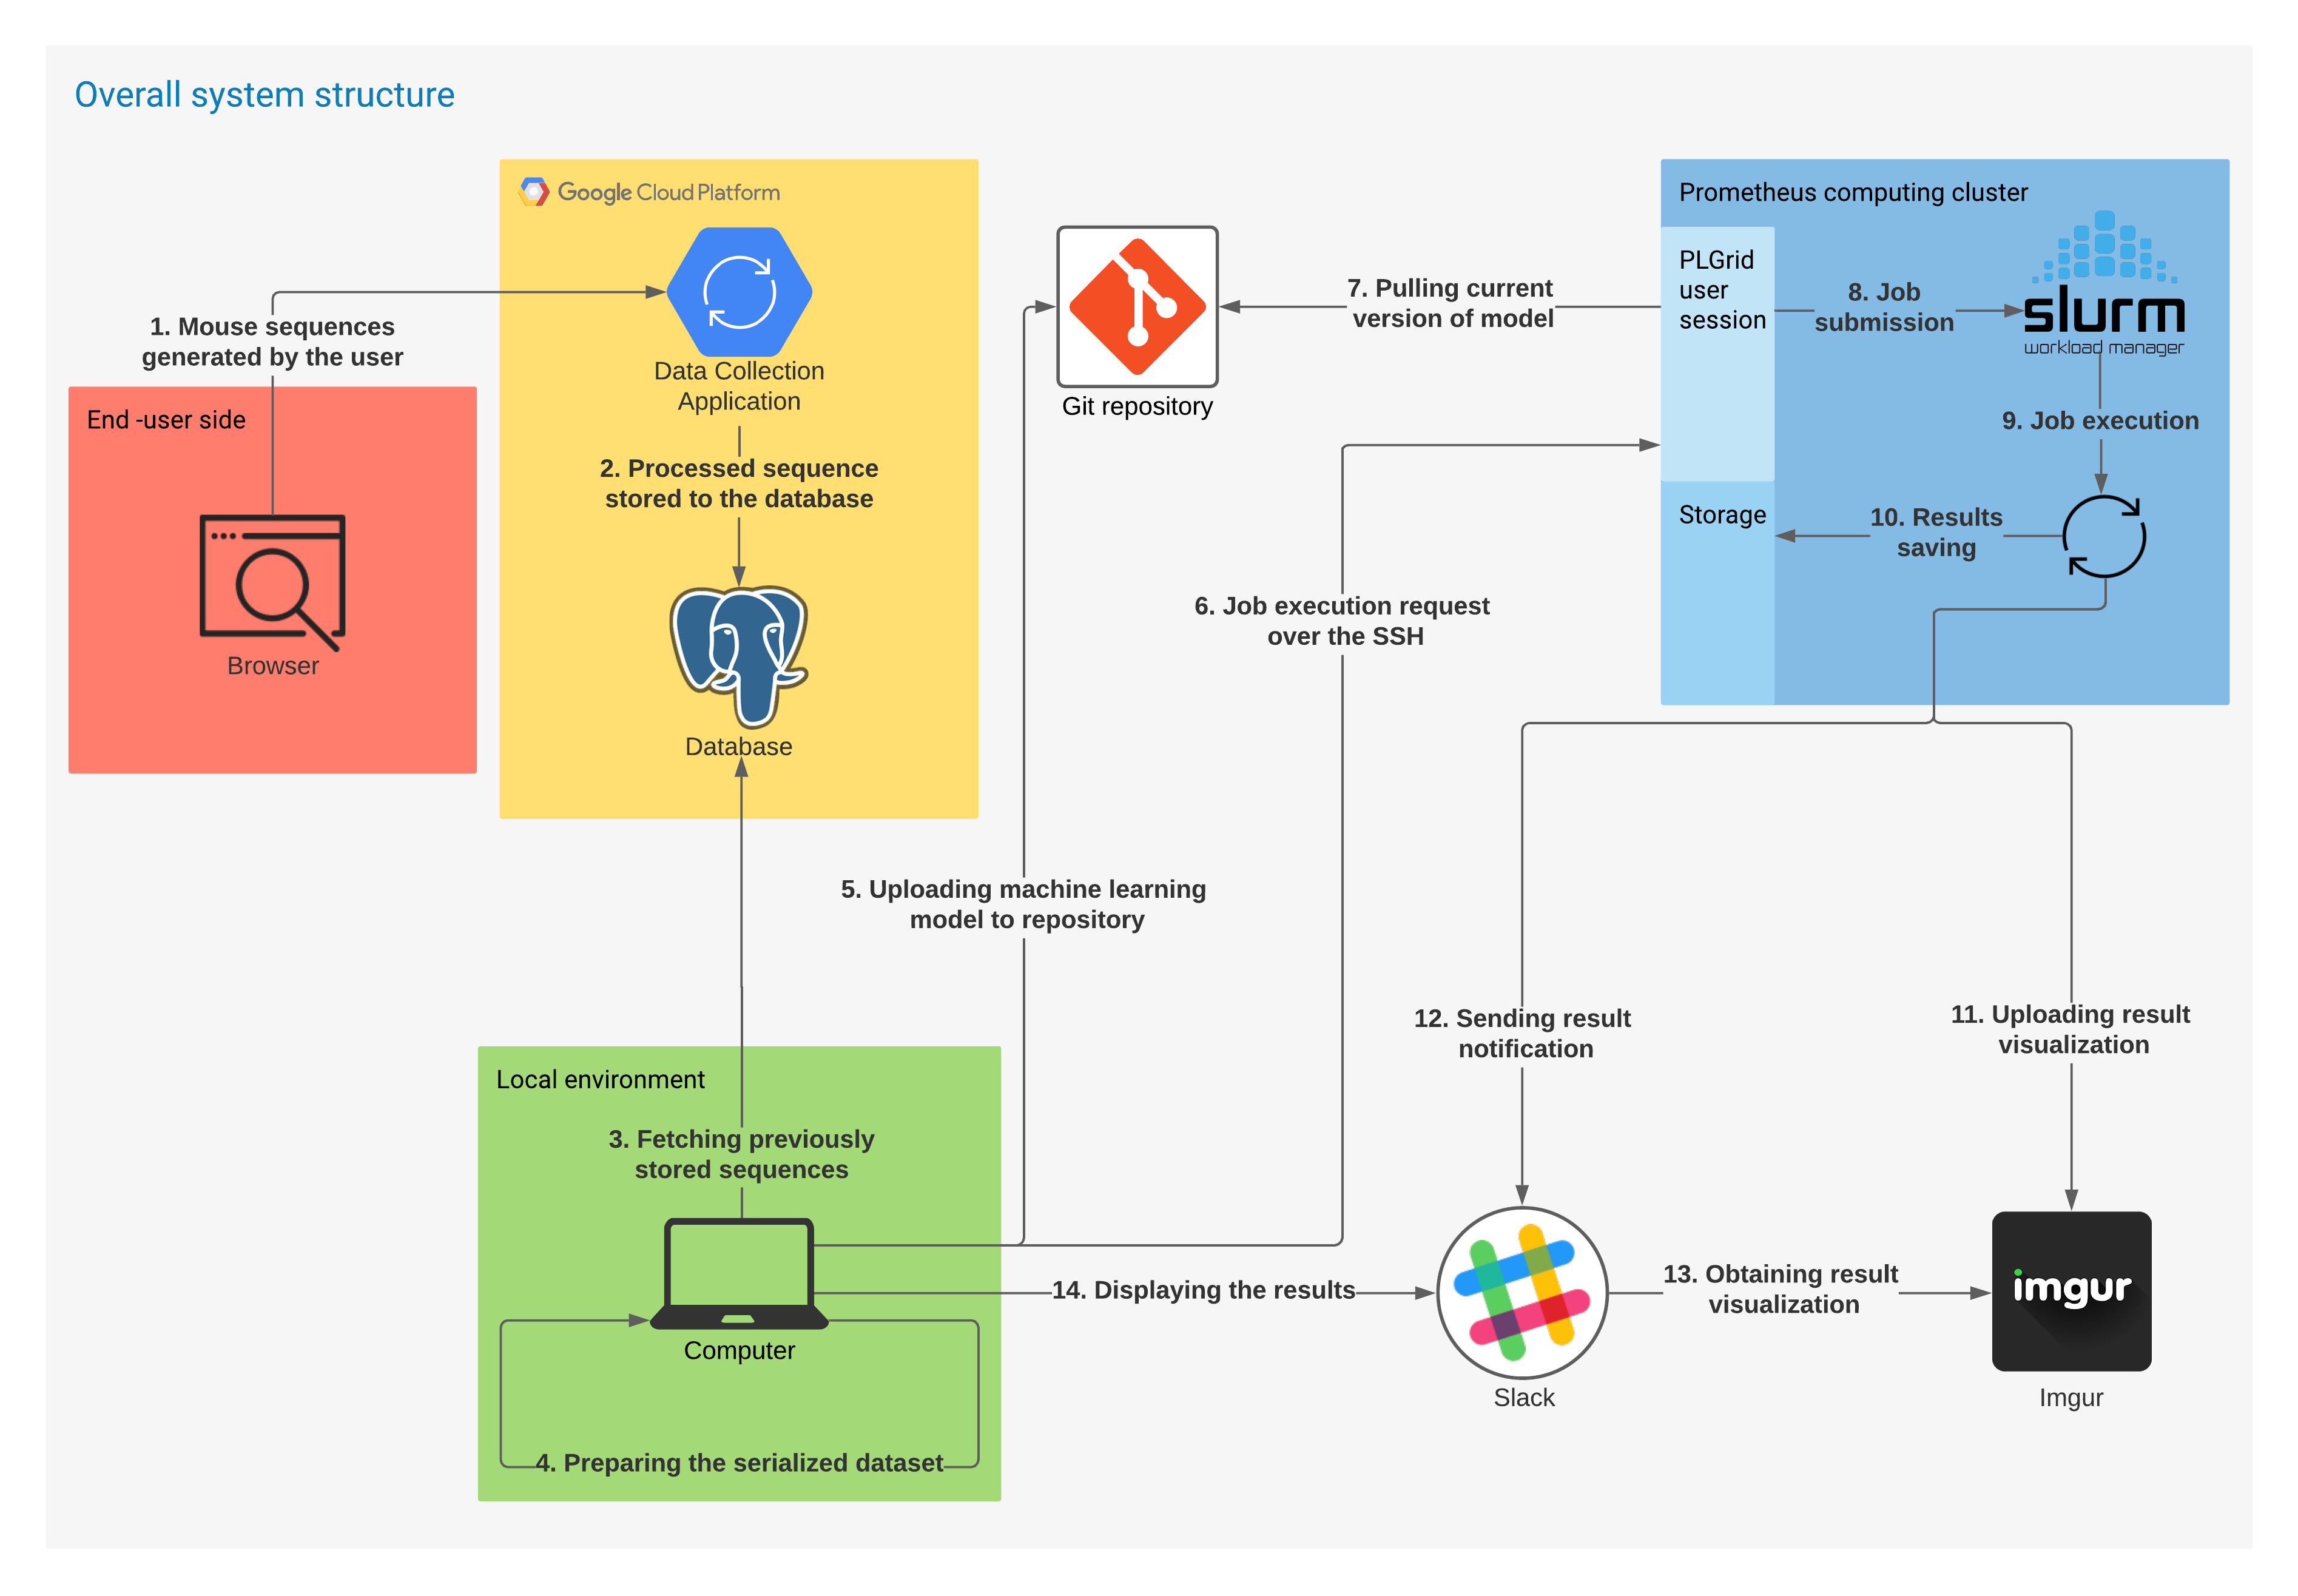
\includegraphics[width=\linewidth]{resources/overall_diagram.png}
    \captionof{figure}{Overall system structure diagram}
    \label{fig:overall_system_structure}
\end{figure}

The entry point for the system is the user's browser that allows the human user as well as a human impersonating bot for access to the prepared website which is hosted on the Internet.
The \mbox{Data Collection}\upperref{itm:data-collection} module which is persisted and operates within a cloud acts as a mouse dynamics data collector, which means that every single mouse event generated by the user on the website is intercepted, transformed and stored in the underlying database (Fig.~\ref{fig:overall_system_structure}, pt. 1 and pt. 2).
The administrator of the presented system is able to retrieve the data from the database in any time (pt. 3).
The downloaded data can be further processed (pt. 4) to the dataset which will be used in machine learning stage.
The administrator of the system should prepare a machine learning model and upload it to the Git repository (pt. 5) which will be then obtained by a computing cluster to perform computation using the model from the observed branch.
Such an approach allows to work on the solution simultaneously by many data scientists and makes it possible to accelerate the research.
The dataset should be uploaded to the computing cluster and persisted in the group's storage that allows using it by many different paralleled computations (not included in the diagram due to decrease of readability).
Each computation is requested from the local computer using prepared Git's `deploy' alias (described in Section~\ref{sec:prometheus-computing-cluster}) that performs a sequence of operations such as establishing the connection to the cluster, fetching the current version of code from the repository and submitting the job to the Slurm\upperref{itm:slurm} workload manager (pt. 6, 7, 8).
The work of the cluster is fully asynchronous because each job is queued and therefore the completion time is unknown.
This is very inconvenient because there is no notification system that allows getting the information about the finished job.
To overcome these limitations, the notification system is proposed as a part of Bot Detection\upperref{itm:bot-detection} module.
The creation of such a system enables the presentation of the results of the computed job in the message as well as the graphs prepared based on the output of the job.
To provide the possibility of sending the images, the notification system uses the external image hosting website called Imgur\upperref{itm:imgur} which allows to upload pictures to the server and host them under the generated \gls{url} (pt. 11).
The results and the graphs are combined into Slack's\upperref{itm:slack} message and then sent to the previously prepared channel by using the webhook \gls{api} (pt. 12, 13).

The further subchapters treat about the implementation details.
At the beginning the Data Collection module is described along with the cloud configuration and performance tests, further, the bot which impersonates the human user and finally the machine learning model alongside the tools such as, among others, a notification module.


\section{Data serialization}\label{sec:data-serialization}
The persisted data from the database is to serve as the input for a machine learning model, however, due to inconvenient usage of SQL queries for such purposes, the serialization tool was developed in order to translate the state of the database records to binary files.
In the presented solution, such files are treated as immutable, so the operation of serialization can be performed only once, which results in the improvement of the required time to read the data by the machine learning model.
Moreover, binary files allow straightforward sending and storing data in external infrastructures, such as PLGrid\footnote{\url{http://www.plgrid.pl/}}, because it does not require maintenance of database engine in that environment.
Such an approach also makes it possible to process data and prepare them in a way that is required by the machine learning model.

To fulfill these requirements, the serializer and deserializer tools were developed for saving sequences in binary files and further reading those data in Python script.
The serialization is performed using a tool written in Go\footnote{\url{https://golang.org/}} and provides additional tuning of resulted binary files and configuration of connection to the database.
Among the others, the tool allows choosing the type of event generated by the user such as mouse click or move, minimum sequence length that should be considered as valid data, minimum screen resolution in order to filter the actions from mobile devices or the time gap between two actions that should be considered as the boundary between two sequences.
The results of such filtration are saved in the chosen directory dividing the output into the user's directories and saving each separate sequence in a single file, so the output consists of many user's directories each containing many single sequence files.
It is also possible to use a so-called one-user mode that enables generating output data only for a single arbitrary chosen user for debugging purposes.

In order to make serialization uncomplicated and transferable between different programming languages, the serialization framework was used.
At the beginning the chosen one was Apache Avro\footnote{\url{https://avro.apache.org/}} which allows to defining the schema in simple JSON file.
The serialization is performed with help of a library that allows reading schema and saving programming language native objects to binary files.
In the presented solution serialization should be performed using the library for Go and the deserialization with support of the library for Python, however, they proved to be incompatible which resulted in errors in deserialized data.

To avoid invalid data and to do not spend too much time on finding the bug in those libraries, another approach was taken by applying the Protocol Buffers\footnote{\url{https://developers.google.com/protocol-buffers}} technology.
Protocol Buffers or simply Protobuf is a method of serializing data to the binary form, but the real advantage of it is official multilingual support by generating a serializing code in required programming language.
Protobuf also requires the definition of a schema like Apache Avro, but unlike Avro, the config file format is developed especially for Protobuf, at the same time it is also readable and effortless to write.
Basing on the created schema the code was generated both for the serializer and the deserializer, but in the case of deserializer, the data is directly read to the Pandas\footnote{\url{https://pandas.pydata.org/}} Dataframe objects, which provides a simple interface to manipulate huge amount of data.
The deserializing tool was designed to work directly in the front of the neural network with additional preprocessing step, therefore it was written in Python to provide flexibility in adapting this feature in further work.
It is also able to read data from the directory tree created by the serializer which enables seamless integration between these two parts.